\subsection*{Partie A}
On note $f$ la fonction définie sur l'intervalle $\left[2 ;+\infty\right[$ par \[f(x)=\ln \left(3 x^{2}+2 x\right).\]

On admet que la fonction $f$ est dérivable sur l'intervalle $\left[2 ; +\infty \right[$ et on note $f'$ sa fonction dérivée.

\begin{enumerate}
	\item Déterminons la dérivée de la fonction $f$.

	$f$ est de la forme $\ln( u)$ avec $u(x) =3 x^{2}+2 x$, on a donc $u'(x)=3\times 2x+2=6x+2$.

	La dérivée de $\ln(u)$ est $\dfrac{u'}{u}$ donc pour tout réel $x$ de l'intervalle $[2 ;+\infty[$, $f'(x) = \dfrac{6x+2}{3 x^{2}+2 x}$.

	$\forall x \in [2 ;+\infty[,  \quad 6x+2 >0$ et $3x^2+2x >0$ donc $f'(x) >0$.

	La fonction $f$ est donc strictement croissante sur l'intervalle $[2 ;+\infty[$.

	\item
	\begin{enumerate}
		\item  Sur l'intervalle $[2;+\infty[$, la fonction $g$ est continue (car dérivable) et strictement décroissante.

		De plus, $g(2) = \ln( 3\times 2^2+2 \times 2)-2 = \ln(16)-2 >0$

		et $\lim\limits_{x \to +\infty} g(x) =- \infty <0$.

		D'après le théorème de la bijection, l'équation $g(x) =0$ admet une unique solution  $\alpha$  sur l'intervalle $[2;+\infty[$.

		Remarque : $g(\alpha) =0 \implies f(\alpha)-\alpha =0 \implies f(\alpha)=\alpha$.

		\item  À l'aide de la calculatrice, on trouve $\alpha \approx 4,05$.

		\item  La fonction $g$ étant strictement décroissante sur $[2 ;+\infty[$ et s'annulant en $\alpha$, on a le tableau de signes suivant :

		\hfill~
		\begin{tikzpicture}
			\tkzTabInit[lgt=3]{$x$/0.6,  signe de $g(x)$/0.6}
			{$2$,$\alpha$,$+\infty$}
			\tkzTabLine{,+,z,-,}
		\end{tikzpicture}
		\hfill~



	\end{enumerate}
\end{enumerate}

\subsection*{Partie B}


\begin{enumerate}
	\item 	Pour tout entier naturel non  nul $n$, posons $P_n$ l'affirmation :\quad \og $2 \leqslant a_{n} \leqslant \alpha$\fg{}.

	Démontrons par récurrence que les affirmations $P_n$ sont toutes vraies.

	\begin{itemize}[label={\textbullet~}]
		\item \textbf{Initialisation :}  Par hypothèse  $2 \leqslant a_{0} \leqslant \alpha$

		Donc que l'affirmation $P_0$ est vraie.

		\item \textbf{Hérédité :} Soit $n$ un entier naturel non nul. On suppose que l'affirmation $P_n$ est vraie, c'est à dire $2 \leqslant a_{n} \leqslant \alpha$\fg{}., montrons que l'affirmation $P_{n+1}$ est vraie, c'est à dire $2 \leqslant a_{n+1} \leqslant \alpha$\fg{}.

		$\begin{aligned}
			P_n \text{ est vraie}
			&\implies 2 \leqslant a_{n} \leqslant \alpha\\
			&\implies f(2) \leqslant f\left(a_n\right)\leqslant f(\alpha)\quad \text{ car la fonction }f \text{ est strictement croissante sur l'intervalle }[2;+\infty[\\
			&\implies   \ln(16) \leqslant a_{n+1} \leqslant \alpha  \quad \text{ car } f(\alpha)=\alpha \text{ et par définition de la suite } \left(a_n\right)  \\
			&\implies 2 \leqslant a_{n+1} \leqslant \alpha \quad \text{ car } \ln(16)\approx 2,77\\
			&\implies P_{n+1}\text{ est vraie.}
		\end{aligned}$
		\item \textbf{Conclusion :} On a montré que l'affirmation $P_0$ est vraie, et que pour un $n$ entier naturel non nul, si $P_n$ est vraie, alors $P_{n+1}$ est vraie.

		En vertu du principe de récurrence, on en déduit que, pour tout entier naturel non nul $n$, l'affirmation est vraie, et donc pour tout entier naturel $n$, on a $2 \leqslant a_{n} \leqslant \alpha$.

	\end{itemize}




	\item  Soit $n$ un entier naturel quelconque :

	$a_{n+1}-a_n= f\left(a_n\right)-a_n = g\left(a_n\right)$.

	Or, d'après la question précédente $a_n \in [2; \alpha]$ et  on a démontré dans la partie A, que la fonction $g$ est positive sur cet intervalle,

	donc $a_{n+1}-a_n\geqslant 0$

	donc la suite $(a_{n})$ est croissante.

	\item  On a montré que la suite $(a_{n})$  est minorée par 2 et qu'elle est décroissante, elle est donc convergente vers une limite $\ell$ telle que $2 \leqslant\ell \leqslant \alpha$.

	\item La suite $(a_{n})$ est définie par une relation de récurrence $a_{n+1}=f(a_n)$ avec $f$ une fonction continue.

	De plus, la suite $(a_{n})$ est convergente vers une limite $\ell$.

	D'après le théorème du point fixe, la limite $\ell$ est donc solution de l'équation $f(x)=x$ soit de l'équation $g(x)=0$.

	D'après la partie A, cette équation admet une unique solution $\alpha$ donc $\ell = \alpha$.

\end{enumerate}

\subsection*{Partie C}

\begin{enumerate}
	\item  Dans la partie B, on a montré que pour tout entier naturel $n$, $a_n < \alpha$.

	On sait que la suite $(b_n)$ est strictement décroissante et qu'elle converge vers $\alpha$ donc pour tout entier naturel $n$, $\alpha \leqslant b_n$

	Donc pour tout entier naturel $n$, on a \quad $a_{n} \leqslant \alpha \leqslant b_{n}$ d'où $a_{n} \leqslant  b_{n}$.

	\item
	
	
	
	
		
		
		
		
		
		
		
		
		
		
		
		
		
		
		
		
			
			
			
			

		\begin{enumerate}
			\item L'instruction \texttt{algo(2)} renvoie : $(9, 4.04)$ arrondi au millième

			\item Cette algorithme calcule les termes successifs des suites  $(a_n)$ et $(b_n)$ jusqu'à ce que

			$b_n-a_n \leqslant 10^{-p}$. Il renvoie donc le 1er rang  $i$ pour lequel $b_n-a_n \leqslant 10^{-p}$ ainsi que le terme $a_i$

			Le premier rang pour lequel on aura $a_n-b_n \leqslant 10^{-2}$ est donc 9 et $a_9\approx 4,04$.
		\end{enumerate}
	\end{enumerate}
